% !TEX TS-program = xelatex
% !TEX encoding = UTF-8
% 2014H1: CITP for CafeOBJ
% toshi.swd@gmail.com
%
\documentclass[a4paper,oneside,10pt,here]{memoir}
\usepackage[hscale=0.76,vscale=0.76]{geometry}
\setlength{\parindent}{0.0cm}
\setlength{\parskip}{1.4ex}
\usepackage{graphicx}
\usepackage{proof}
\usepackage{fancyvrb}
\usepackage{amssymb}
\usepackage{bussproofs}

%%% Japanese
\usepackage{fontspec}
\usepackage{indentfirst}
\setmainfont[Ligatures=TeX]{Meiryo}
\setsansfont[Ligatures=TeX]{Hiragino Kaku Gothic ProN W3}
\setmonofont[Ligatures=TeX]{Osaka-Mono}
\XeTeXlinebreaklocale "ja"
\XeTeXlinebreakskip=0em plus 0.1em minus 0.01em
\XeTeXlinebreakpenalty=0
\renewcommand{\baselinestretch}{1.4}
\settowidth{\parindent}{あ}
%%%%
\usepackage{dcolumn,hhline,colortbl}
\usepackage[table]{xcolor}
%%%%% 色付表
\newcolumntype{G}{%
  >{\columncolor[gray]{0.9}}c}
\newcolumntype{O}{%
  >{\columncolor{orange}}c}
\newcolumntype{M}{%
  >{\columncolor{green}}c}
\newcolumntype{Y}{%
  >{\columncolor{yellow}}c}
\newcolumntype{C}{%
  >{\columncolor{cyan}}c}
%%%% hyperref
%\usepackage[dvipdfm,colorlinks=true,linkcolor=blue]{hyperref} 
\usepackage[colorlinks=true,linkcolor=blue]{hyperref} 
%%%%%%%%%%syntax
\makeatletter
% terminal - used for terminal symbols, argument is characters appear in sf.
\def\sym#1{\textsf{#1}\null}
% nonterm - used for non terminal symbols, argument is characters typed with
%           italic face.
\def\nonterm#1{\textit{#1}\null}
%%%%%
% syntax ... endsyntax
\def\xstrut{\relax\ifmmode\copy\strutbox\else\unhcopy\strutbox\fi}
\def\syntax{\syntaxoutnonbox\halign\bgroup
    \xstrut$\@lign##$\hfil &\hfil$\@lign{}##{}$\hfil
    &$\@lign##$\hfil &\qquad\@lign-- ##\hfil\cr}
\def\endsyntax{\crcr\egroup$$
  \global\@ignoretrue
}
\def\syntaxoutnonbox{\xleavevmode$$
    \parskip=0pt\lineskip=0pt
    \def\\{\crcr}% Must have \def and not \let for nested alignments.
    \everycr={\noalign{\penalty10000}}
    \tabskip=0pt}
\def\xleavevmode{\ifvmode\if@inlabel\indent\else\if@noskipsec\indent\else
    \if@nobreak\global\@nobreakfalse\everypar={}\fi
    {\parskip=0pt\noindent}\fi\fi\fi}
\def\@but{\noalign{\nointerlineskip}}
\def\alt{{\;|\;}}
\def\seqof#1{\mbox{\textbf{\{}}\;{#1}\;\mbox{\textbf{\}}}}
\def\optn#1{\textbf{[}\;{#1}\;\textbf{]}}
\def\synindent{\;\;\;}
%%%%
\def\SP{\mathit{SP}}
\def\PR{\mathtt{PR}}
\def\Sig{\mathbb{S}\mathit{ig}}
\def\tr{\mathtt{true}}
\def\fs{\mathtt{false}}
\makeatother
%%%
%%%% numbering
%%% ToC down to susubsections
\settocdepth{subsubsection}
%%% Numbering down to sections
\setsecnumdepth{subsection}
%%% 名前定義を適当に
\def\figurename{{図}}
\def\tablename{表}
\def\contentsname{目次}
\def\listfigurename{図目次}
\def\listtablename{表目次}
\def\refname{参考文献}
\def\bibname{参考文献}
\def\indexname{索引}
\def\appendixname{付録}
%%%%%%%%%% Verbatim
\DefineVerbatimEnvironment%
{simplev}{Verbatim}
{fontsize=\small}
\DefineVerbatimEnvironment%
{examplev}{Verbatim}
{frame=leftline,fontsize=\small}
%%%%%%%%%%
\definecolor{shadecolor}{gray}{0.9}
\newenvironment{vvtm}%
{\parskip=0pt\lineskip=0pt\begin{center}\begin{minipage}{0.8\textwidth}\begin{snugshade}}%
  {\end{snugshade}\end{minipage}\end{center}}
%%%
\usepackage{float}
\begin{document}
\headstyles{default}
\tightlists
%\midsloppy
\sloppy
\raggedbottom
\chapterstyle{ell}
%%%%%%%%
\frontmatter
\pagestyle{empty}
% 表紙 %%%%%%%%%%%%%%%%%%%%%%%%%%%%%%%%%%%%%%%%%%%%%%%%%%%%%
\title{証明譜作成支援機構 CITP for CafeOBJ}
\vfill
\author{澤田 寿実\\
  (株) 考作舎\\
  tswd@kosakusha.com}
\date{2015/3/10}
\maketitle
\vfill
\begin{center}

\includegraphics[scale=0.2]{kosakusha2_gray.pdf}
\end{center}
\vfill
\thispagestyle{empty}
\newpage
%%%%%%
\mainmatter
\pagestyle{plain}
\pagenumbering{arabic}
% 構成 %%%%%%%%%%%%%%%%%%%%%%%%%%%%%%%%%%%%%%%%%%%%%%%%%%%%%
\tableofcontents
\EnableBpAbbreviations
\newpage
\chapter{CITP for Cafe の新規コマンド}\label{chap:new-commands}
本章では CITP for Cafe で新たに導入されたコマンド群の仕様について述べる.

\section{用語}\label{sec:terms}
表\ref{table:terms}に以下で使用するいくつかの用語の定義を示す.

\begin{table}
\caption{用語の定義}
\label{table:terms}
\begin{center}
\begin{tabular}[tbhp]{|l|p{0.6\textwidth}|}\hline
用語 & 定義 \\\hline\hline
文(sentence)   & 自由変数を含まない(条件付き)等式($t = t' if C$) あるいは、(条件付き)遷移規則 ($t \Rightarrow t'$).
CafeOBJ の等式宣言や遷移規則宣言のフォームで表記する. \\\hline 
文脈(context) & 証明を実施するモジュール.\\\hline
ゴール(goal) & 四つ組 $<M,G,C,H>$. 文脈($M$)とそこで証明したい文の集合($G$),
証明に際して使用した戦略(tactic)により導入された定数(constants)の集合($C$)と
仮定(hypothesis)$H$(文の集合).単に証明対象とする文(の集合)をゴールと呼ぶことがある.\\\hline
戦略(tactic) & tactic.証明で用いる演繹規則およびそれらを組み合わせたものを戦略(tactic)と呼ぶ.\\\hline
基底項(ground term) & 変数を含まない項. \\\hline
\end{tabular}
\end{center}
\end{table}

\section{証明の開始(ゴールの設定)} \label{sec:start-proof}
ある特定のモジュール $M$ を文脈として,その中で証明したい文の集合 $G$ がすべて
成立することを演繹規則(戦略)を順次適用することによって証明することが本システムの
目標となる.

\begin{itemize}
\item 証明を開始するには,証明を行う文脈を設定し証明したい文の集合を宣言する.\\
  文脈の設定は,既存の CafeOBJ コマンド \verb|select <ModuleExpression> .| あるいは \verb|open <ModuleExpression> .|
  によって行う.
\item 証明を実施する文脈の設定後,下に示す \verb|:goal| コマンドによって証明したい文の集合を指定する.\\
  \begin{vvtm}
    \begin{simplev}
    goal コマンド ::= :goal { <sentence> .  ...  <sentence> . }      
    \end{simplev}
  \end{vvtm}
  \verb|sentence| は,CafeOBJ の(条件付き)等式あるいは(条件付き)遷移規則のいずれかで
  表記する.
\end{itemize}
\subsubsection{文脈とゴールの設定例}
\begin{vvtm}
  \begin{simplev}
 select CLOUD . 
 :goal {
  ceq [inv1 :nonexec]: true = false if statusp(S:Sys,I:Client) = updated /\
                                        statusc(S:Sys)= idlec .
  ceq [inv2 :nonexec]: true = false if statusp(S:Sys,I:Client) = gotval /\ 
                                       statusc(S:Sys)= idlec .
  ceq [inv3 :nonexec]: true = false if statusp(S:Sys,J:Client) = updated /\
                                       statusp(S:Sys,I:Client) = gotval .
  ceq [inv4 :nonexec]: true = false if (I:Client ~ J:Client) = false /\
                                       statusp(S:Sys,J:Client) = gotval /\ 
                                       statusp(S:Sys,I:Client) = gotval .
  ceq [inv5 :nonexec]: true = false if (I:Client ~ J:Client) = false /\
       statusp(S:Sys,J:Client)= updated /\ statusp(S:Sys,I:Client)= updated .}
  \end{simplev}
\end{vvtm}

\section{証明木の構造}\label{sec:proof-struct}
ここでは他のコマンドを説明する前に,CITP for CafeOBJ の構成する
証明木(proof tree)の構造について説明する.

証明木は全体としてゴールをノードとする有向の木構造(directed tree structure)を持ち,
各枝(branch)はゴールに対して適用した戦略をラベル(label)が付加されている.
あるゴール$G$に対してある戦略$T$を適用すると,
一般的に複数のゴール$G_1, G_2, \ldots, G_n$ が生成されるが,
これら $G_i$ をもとのゴールの子ゴールと呼ぶ.
$G$ から各 $G_i (i = 1 \cdots n)$ への枝は,全て適用した戦略$T$によるラベル $T$を持つ.

以下この一般的な証明木の構造をより具体的に述べる.
以下では,ゴールと証明木のノードを区別せずに用いる.

\begin{itemize}
\item :goal コマンドによって設定されたゴールを初期ゴールとする.
\item あるノード(ゴール)に対して戦略 $T$ の適用によって新たなゴールが生成された場合,
  それらをそのノードの子ノードとする.これら子ノードへの枝はラベル $T$ を持つ.
\item 各ゴールには次のように名前が付加される:
  \begin{itemize}
    \item 初期ゴールには root という名前が付けられる.
    \item root 直下のゴールには自然数 $1, 2, \ldots n$ と名前が付けられる.
    \item 以下,あるゴールの名称が N であったとすると,そのゴールには
      N-1, N-2, $\ldots$ N-m のように名前が付けられる.
  \end{itemize}
\end{itemize}
\begin{figure}[hbt]
  \centering
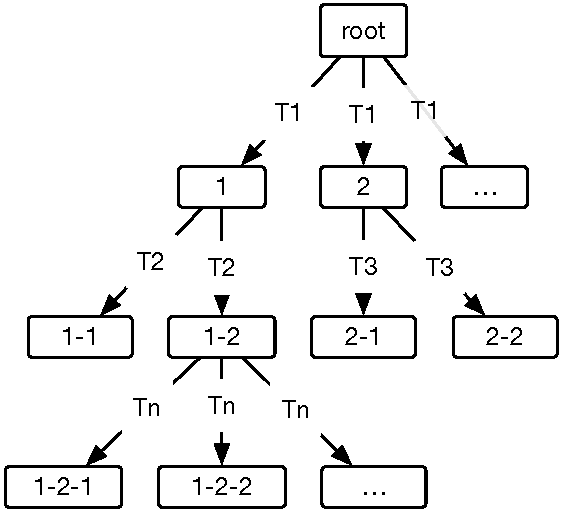
\includegraphics[scale=1.0]{proof-tree.pdf}  
  \caption{証明木}
  \label{fig:proof-tree}
\end{figure}

上のような構造の証明木において, ``ゴールが証明される''とは以下の事を言う:
\begin{itemize}
\item あるゴールの子ゴールが全て証明されたとき,そのゴールも証明される
\item ここで ``証明される'' とは以下の事を言う
  \begin{itemize}
  \item 文が充足(satisfied)される
  \item 矛盾(contradiction)が発見される: すなわち
    \begin{itemize}
    \item その文脈において true = false が演繹可能(deducible)となる
    \item 遷移的な関係で矛盾が生ずる.例えば $X < Y < Z$ の時に
      $Z \le Y$ が演繹できる.
    \end{itemize}
  \item これらのいずれかが成立した時,そのゴールに含まれる当該文はゴールから
    取り去られる (dischage されると言う).
  \item ゴールから証明対象の文がすべてなくなった時,
    そのゴールは証明されたと言う.
  \end{itemize}
\end{itemize}

\section{戦略の適用}\label{sec:apply}

\begin{itemize}
\item 初期ゴールが設定された後では,:apply コマンドによって,指定の戦略をゴールに適用できるようになる.
  ゴールが設定されていない場合,:apply コマンドの適用はエラーとして扱う.
\item 構文
  \begin{vvtm}
    \begin{simplev}
    apply コマンド ::= :apply [ to <GoalName> : ] (<Tactic> ... <Tactic> )
    <GoalName>     ::= ゴールに付与された名前
    <Tactic>       ::= SI | CA | TC | IP | RD
    \end{simplev}
  \end{vvtm}

\item \verb|<Tactic>| の指定で,大文字と小文字の区別はしない.
\item \verb|to <GoalName>| が省略された場合は,現在のデフォルトゴール(後述)に対して適用される.
\end{itemize}
各戦略の意味と挙動については後述する.

\subsubsection{戦略の適用順序}

\begin{figure}[htbp]
\begin{center}
  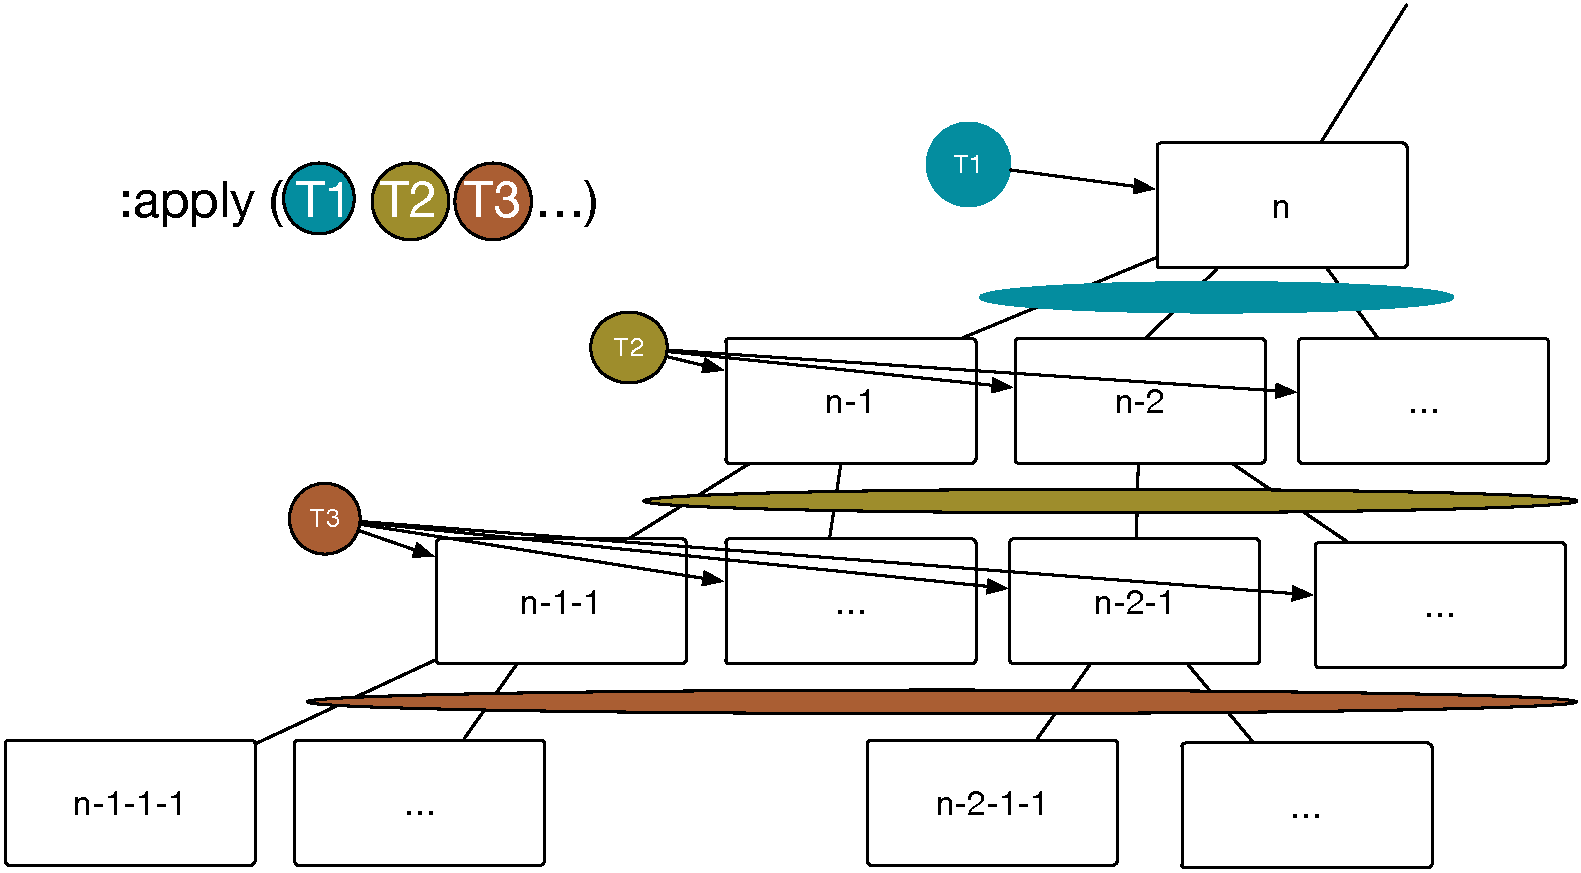
\includegraphics[scale=0.4]{apply-order.pdf}
\end{center}
\caption{戦略の適用順序}
\label{fig:apply-tactic}
\end{figure}
図~\ref{fig:apply-tactic} に,あるゴール $n$ に対して一連の戦略 $T_1 T_2 \ldots T_n$ を
適用した際に,これらの戦略がどのように適用されるかを示す.
一般にある戦略 $T_i$ をゴール $N$ に適用した場合,戦略によって複数のゴールが生成される.
:apply コマンドに一連の戦略 $T_1 T_2 \ldots T_n$ が指定され,ゴール $N$ に適用されたとする.
このとき最初の戦略 $T_1$ によって複数の小ゴール $N_1 \ldots N_m$ が生成されたとした時,
次の戦略 $T_2$ はこれらの小ゴール全てに対して適用される.以下同様である.

\subsubsection{戦略}
CITP for Cafe で提供される戦略を表~\ref{tab:tactics} に示す.
各戦略の具体的な挙動については,後に章を改めて説明する.

\begin{table}
\label{tab:tactics}
\caption{戦略一覧}
\begin{center}
\begin{tabular}[tbhp]{|l|l|}\hline
戦略 & 演繹規則 \\\hline\hline
SI & Simultaneous Induction (同時帰納法) \\\hline
CA & Case Analysis (場合分け)\\\hline
TC & Theorem of Constants  \\\hline
IP & Implication \\\hline
RD & Reduction (簡約化) \\\hline
\end{tabular}
\end{center}
\end{table}

\subsubsection{自動戦略} 
経験則から一般的に有効(うまく証明ができることが多い)と考える事のできる一連の戦略を予め用意し,
これを簡便に使用できると便利である.
このためにコマンド :auto が用意されている.

\begin{itemize}
\item 構文:
  \begin{vvtm}
    \begin{simplev}
  auto コマンド ::= :auto      
    \end{simplev}
  \end{vvtm}
\item \verb|:auto| は \verb|:apply (SI CA TC IP RD) | と等価である.
\end{itemize}

\section{ターゲット・ゴール}\label{sec:default-goal}
現在戦略適用の対象となっているゴールを,ターゲット・ゴールと呼ぶ.

\begin{itemize}
\item 初期のゴールが \verb|:goal| コマンドによって設定された直後は 
  \verb|root| がターゲット・ゴールである.
\item ある戦略をゴールに適用した後は,証明木の構造上最も左の
  末端ノードがターゲットゴールとなる.
\item ターゲット・ゴールは,\verb|:select| コマンドによって陽に設定することが可能である.
\item 構文:
  \begin{vvtm}
    \begin{simplev}
  :select コマンド ::= :select <GoalName>      
    \end{simplev}
  \end{vvtm}
\end{itemize}

\section{暗黙的戦略}\label{sec:implicit-tactic}
\verb|:apply| コマンドによって指定することはできないが,
システム内部で自動的に適用される戦略がある.
以下ではこれらについて説明する.

\begin{itemize}
\item ある戦略を適用した後にゴールに含まれる証明対象の文に
  含まれる基底項(ground term)は全て既約形(normal form)にされる.
  その後,以下の戦略が暗黙的に適用される.
\end{itemize}

\subsubsection{CT: contradiction の検知}\label{sec:CT}
ゴール 内で true = false が演繹可能かどうかを調べる.

\begin{prooftree}
  \AXC{$\SP \vdash \tr \Rightarrow \fs$}
  \LeftLabel{[CT]}
  \UIC{$\SP \vdash \rho$}
\end{prooftree}

これが可能な場合,矛盾なので任意の証明対象の文が discharge される.

\subsubsection{VD: 文が成立することの検査}\label{sec:VD}

証明対象の文が成り立つかどうか(valid)かを調べる.
具体的には,証明対象の文がすべて基底項から構成されている場合に以下を行う.
証明対象の文を \texttt{ l = r if C} とする:
\begin{enumerate}
\item 条件部 \texttt{C} の既約形(normal form)を求める.
  結果が \texttt{true} ならば次へ進む(条件部が存在しない場合は \texttt{true} とみなされる).
  結果が \texttt{true} でなければ文はまだ成立しないとみなす.
\item 文の左辺 \texttt{l} の規約形を求める.
\item 文の右辺 \texttt{r} の規約形を求める.
\item 左右両辺の既約形が「等しい」かどうかを調べる.
  ここで,等しいとは以下のことを言う:
    \begin{itemize}
    \item 項の形が同じ.
    \item 項のトップオペレータが(associative, commutative)などのセオリー属性を持っていた場合,
      その意味で等しい.
    \end{itemize}
\item 等しければ成立する.等しく無ければ成立しない,とする.
\end{enumerate}

\begin{itemize}
\item CT と VD は,IP および TC で得られたゴールに対して自動的に適用される.
\item CA を適用したがケースが生成されなかったゴール対しても CT と VDが適用される.
\end{itemize}

\subsubsection{LE: 順序関係で互いに矛盾する公理の存在有無を調べる}\label{sec:LE}

\begin{itemize}
\item 現在は組込の INT モジュールで定義されている,整数の大小関係
  \verb|<| と \verb|<=| についてのみ検査が実施される.
\item LE は,CA のケースわけによって生成された公理(仮定)を検査対象とする.
\end{itemize}

\begin{prooftree}
  \AXC{}
  \LeftLabel{[LE]}
  \UIC{$\SP \vdash \rho$}
\end{prooftree}


\section{各戦略の挙動}\label{sec:tactic-behaviour}
本章では先に述べた各戦略の挙動について述べる.

\subsection{SI: Simultaneous Induction}\label{sec:SI}

\begin{prooftree}
\AXC{$\{\SP\vdash^{sp} (\forall Y)\theta(\varepsilon)\;|\; \theta : X \rightarrow T_{\Sigma^{c}}, Y : \mathtt{finite}\}$}
\LeftLabel{[conAbst]}
\UIC{$\SP\vdash^{sp} (\forall X)\varepsilon$}
\end{prooftree}
ここで $\Sigma = \Sig(\SP)$,$\Sigma^{c}\subset\Sigma$ は構成子からなる部分シグニチャである.
また $\theta : X\rightarrow T_{\Sigma^{c}}(Y)$ は $\Sig(\SP)$-置換である.
上の規則はもし $\varepsilon$ が $X$ に含まれる変数の全ての可能な%
instantiationについて成り立つなら $(\forall X)\varepsilon$ が成り立つことを意味する.

[conAbst] は実用的な観点からは使用するのが難しい.
何故ならルールのインスタンスが無限にあり得るからである.
その代わりに下の帰納的演繹によってこれを模倣する事が出来る.

\begin{prooftree}
\AXC{$\SP' =_{def} \PR(\SP,\{\{x\}_{s}\}) \cup \{(\forall\{\})\varepsilon\}$}
\noLine
\UIC{$\SP' \vdash (\forall Z^{f})\varepsilon[x\leftarrow f(z_1,\ldots,z_{i-1},x,z_{i+1},\ldots z_n)]\;\; f\in F^{c}_{*s}\}$}
\LeftLabel{[Ind]}
\UIC{$\SP\vdash^{sp}(\forall\{\{x\}_{s}\})\varepsilon$}
\end{prooftree}
\begin{itemize}
\item [Ind]は構成子ベースの帰納的演繹を定式化したものである.
\end{itemize}

\begin{itemize}
\item 戦略 SI は上の Ind を複数の帰納変数に対して同時に適用可能なよう拡張したものである.
指定した帰納変数(induction variables)に対して以下を行う.
  \begin{itemize}
    \item ベースケース
    \item 帰納法の仮定+ステップケース
  \end{itemize}
  それぞれに対応した新たなゴールを生成する
\item induction variables は \verb|:ind on| コマンドによって指定する.
  \begin{vvtm}
    \begin{simplev}
    :ind コマンド ::= :in on ( <変数> ... )      
    \end{simplev}
  \end{vvtm}
   \verb|<変数>| は on-the-fly の変数宣言形式で指定する.
 \item \verb|:ind| コマンドで指定した変数に対応するソートが,構成子を
   持たないソートであった場合はエラーとする.
 \item 帰納法の仮定や,証明対象とするステップケースの文では,
  帰納法による定数が必要となるが,それらは次のようにして生成する.
  \begin{itemize}
    \item \verb|帰納変数名#ソート名| という名前のオペレータを導入
    \item このオペレータを用いて(定数)項を生成する
    \end{itemize}
  例えば,帰納変数として \verb|I:Foo| が指定された場合,
  導入される定数名は \verb|I#<ソート名>| となる.
  <ソート名> は文脈に応じて適切なソートが選択される.
\end{itemize}

\subsection{TC: Theorem of Constants}\label{sec:TC}
\begin{prooftree}
\AXC{$\PR(\SP,Y)\vdash^{sp} (\forall\{\})\varepsilon$}
\LeftLabel{[TC]}
\UIC{$\SP\vdash^{sp}(\forall Y)\varepsilon$}
\end{prooftree}

この演繹規則は全称的に束縛された変数に関する推論を行う際に,
定数を代わって使用しても良いとするものであり,
従来よりCafeOBJの書き換えエンジンを利用した証明で通常利用されている技法である.

CITP CafeOBJ ではこの演繹規則に対応するものを戦略として提供する.
[TC]によって新たに導入する定数名は,既存の定数名と衝突が無いように考慮し,
規則的に命名するものとする.

\begin{itemize}
\item 適用先のゴールに複数の証明対象の文が含まれている場合は,
    それ毎に別々の小ゴールを作成し,分配する.
\item 以下各ゴールに対して以下を実施する.
  \begin{itemize}
  \item 証明対象の文に含まれる変数を対応するソートの定数で置き換える
  \end{itemize}
\item 定数は次のように新たなオペレータを導入することによって作成する
  \begin{itemize}
  \item \verb|変数名@ソート名| という名前のオペレータを導入
  \item このオペレータを用いて(定数)項を生成する
  \end{itemize}
  例えば,変数 X がソート Foo の変数であった場合,導入されるオペレータは
\begin{verbatim}
   op X@Foo : -> Foo .
\end{verbatim}
  のように宣言されたのと等価である.
\item 上記を実施した後,生成したゴールに対して暗黙的戦略 CT および ST を適用する.
\end{itemize}

\subsection{IP: Implication}\label{sec:IP}
\begin{prooftree}
\AXC{$(\Sigma,E\cup\{(\forall\{\})t_1=t'_1,\ldots,(\forall\{\})t_n=t'_n)\vdash^{sp}(\forall\{\}t=t')$}
\LeftLabel{[IP]}
\UIC{$(\Sigma,E)\vdash^{sp}(\forall\{\}) t = t'\; \mathtt{if}\; \{t_1=t'_1,\ldots,t_n=t'_n\}$}
\end{prooftree}

条件付き等式で条件部が基底項の場合,それらを新たな公理として導入し,
条件部を取り去ったゴールを新たなゴールとしても良い事を [IP] は示している.

[IP] についても CITP for CafeOBJ の提供する演繹規則として提供する.
条件部が複数の atom の連結 ($\wedge$ で結ばれた複数の条件)の場合は,
それらを別々の複数の公理として導入する.

\begin{itemize}
\item 適用先のゴールに複数の証明対象の文が含まれている場合は,
  それ毎に別々の小ゴールを作成し,分配する.
\item 以下,各ゴールに対して以下を実施する.
\item 証明対象の文が \verb|ceq T = T' if C| または
  \verb|ctrans T => T' if C| の形,かつ
\item C が基底項の場合に以下を行う
  \begin{itemize}
  \item \verb|C| を公理として追加
  \item 元の証明対象から条件部を削除したものを新たな証明対象の文とする
  \item \verb|C| が複数の条件が \verb|c1 /\ c2 ... /\ cn| のように,\verb|/\| で
    結合された形の場合は分離し,個々の \verb|c1| $\ldots$ \verb|cn| を
    公理として導入する.
  \end{itemize}
\item 以上を実施した後,生成されたゴールに対して暗黙の戦略 CT および ST を適用する.
\end{itemize}

\subsection{CA: Case Analysis}\label{sec:CA}

\begin{prooftree}
\AXC{$\{\PR(\SP,Y) \cup \{ u = t\}\vdash^{sp} e\;|\; t\in T_{\Sigma^{c}}(Y)_{S_{c}}, Y:\mathtt{finite}\}$}
\LeftLabel{[split]}
\UIC{$\SP\vdash^{sp} e$}
\end{prooftree}

\begin{prooftree}
\AXC{$\SP\cup\{u = \mathtt{true}\}\vdash^{sp} e$}
\AXC{$\SP\cup\{u = \mathtt{false}\}\vdash^{sp} e$}
\LeftLabel{[splitBool]}
\BIC{$\SP\vdash^{sp} e$}
\end{prooftree}

これらは網羅的な場合分けの必要性について定式化したものである.
これについては証明の文脈となっている仕様や%
証明の対象としている項により異なり,%
一般的な生成スキームを与える事は困難である.

そのため,場合分けを実施する上での各ケースを利用者が公理によって明示的に指示し,
システムがそれをベースに必要な場合分けを実施するものとする.
この仕様は Maude の CITP システムに習ったものである.

CA は次のように動作する:
\begin{enumerate}
\item 証明対象の文から基底項 $G_1, \ldots, G_n$ を取り出す.
\item 文脈となっているモジュールから,ラベルとして先頭が ``CA'' で始まる
  公理の集合 $Ac$ を求める.
\item 各 $G_i (1\le i \le n)$ について,その真部分項が $Ac$ に含まれる公理の
  どの左辺とも照合しない基底項の集合 $Gs$ を得る.
\item 各 $g_j \in Gs$ について,各 $(\mathtt{l\; =\; r\; if\; C}) \in Ac$ との間で
  以下を計算する.
  \begin{enumerate}
  \item 基底項 $g_j$ に関するケースの集合 $C_j$ を空集合にセットする.
  \item $\sigma(g_j) = \mathtt{l}$ となる置換 $\sigma$ が存在したら,
    $\sigma(C)_j$ を $Cs_j$ に追加する.
  \end{enumerate}
  各 $Cs_j$ は基底項 $g_j$ に関するケースの集合となっているので,
  これらの全ての組み合わせ $CS_1 \times S_2 \times \cdots\S_m$ を計算し,
  全ての可能なケースの組み合わせを求める.
  \item 上で得られた各組み合わせごとに,新たな子ゴールを生成し,
    そのゴールへケースを公理として追加する.
\end{enumerate}
冗長なケースの生成があり得るための,それらを検査して取り除く事は
実装に際して最適化の意味で実施するものとする.

\begin{itemize}
\item 上で述べた CA 処理を実施するする前に,適用対象のゴールに複数の
  証明対象の文が含まれていたら,それらを個々の小ゴールに分配し,
  その後,上の CA 処理を実施する.
\item CA で生成された各ゴールに追加された公理については,
  暗黙的戦略 LE による整数の順序関係に関する矛盾の有無を検査し,
  矛盾が発見されたら直ちにそのゴールを discharge する.
\end{itemize}

\subsection{RD: Reduction}\label{sec:RD}

戦略 RD は,先に暗黙的戦略(\ref{sec:implicit-tactic}で述べた CT と VD を実行するものである.

\section{その他の新規導入コマンド}\label{sec:other-commands}

\subsection{:init コマンド} 

\begin{itemize}
\item \verb|:init| コマンドは証明の途中で lemma の導入と初期化を行うためのコマンドである.
\item 構文
  \begin{vvtm}
    \begin{simplev}
 :init コマンド ::= :init "["<label>"]" by <Substitution>
                 |  :init "(" <axiom> ")" by <Substitution>
 Substitution ::= "{" <Variable> <- <Term> ; ... <Variable> <- <Term> ; "}"
    \end{simplev}
  \end{vvtm}
\item これを実行することによって,\verb|<label>| で指定されたラベルを持つ公理,
  あるいは "(" と ")" で囲まれた公理に含まれる変数を \verb|Substitution| で
  示された変数置換によって初期化した公理を,ターゲット・ゴールの公理として追加する.
\item 追加する公理は,後で見た時に :init コマンドによって導入された事が分かるよう
 \texttt[INIT] というラベルを付加する.
\end{itemize}

\subsubsection{:init コマンドの例}

文脈となっているモジュールに,次のような公理があったとする.
\begin{verbatim}
ceq[inv3 :nonexec]: true = false if statusp(S:Sys,J:Client) = updated /\ 
                                              statusp(S:Sys,I:Client) = gotval .
\end{verbatim}
これに対して下のような :init コマンドを適用できる.
\begin{verbatim}
  :init [inv3] by {S:Sys <- S#Sys ; J:Client <- I@Client ; I:Client <- S#Client ;}
\end{verbatim}
これを実行することによって,新たな公理
\begin{verbatim}
ceq [INIT]: true = false if statusp(S#Sys, I@Client) = updated /\
                                  statusp(S#Sys, S#Client) = gotval .
\end{verbatim}
が,追加される.

\subsection{:roll back コマンド}

\begin{itemize}
\item :roll back は,現在のターゲット・ゴールに対して適用された,直前の戦略を
  キャンセルする.
\item 構文
  \begin{vvtm}
    \begin{simplev}
      :roll back コマンド ::= :roll back
    \end{simplev}
  \end{vvtm}
\item このコマンドの実行により,ターゲット・ゴールは証明木から削除される.
\end{itemize}

\subsection{:cp コマンド}

\begin{itemize}
\item :cp コマンドは指定した2つの文のクリティカルペアを求め,
  利用者に提示する.
\item 利用者はそれに対して,次節で述べる :equation コマンド等を用いて,
  それを公理としてターゲット・ゴールへ追加する事ができる.
\item 構文
  \begin{vvtm}
    \begin{simplev}
      :cpコマンド ::= :cp <Sentence> >< <Sentence>
      <Sentence>  ::= "["<Label>"]" | "(" <axiom> . ")"
    \end{simplev}
  \end{vvtm}
\item \verb|<Sentence>| は,文脈モジュールで宣言されている公理のラベルを
  \verb|<Label>| で指定するか,あるいは CafeOBJ の公理宣言フォームを
  "("と")"で囲んで記載する.
\end{itemize}

\subsubsection{:cp コマンドの使用例}
この例は,直接文を CafeOBJ の公理の宣言記法で記述しクリティカル・ペアを
求めている例である.
\begin{vvtm}
  \begin{simplev}
:cp (ceq top(sq(S@Sys)) = I@Pid if pc(S@Sys,I@Pid) = cs .) 
    >< 
    (ceq top(sq(S@Sys)) = J@Pid if pc(S@Sys,J@Pid) = cs .)
  \end{simplev}
\end{vvtm}

\subsection{:equation/:rule コマンド}

\begin{itemize}
\item これらのコマンドは :cp コマンドで得られたシステムからのクリティカル・ペアの
  提示に対する,利用者の回答として使用される.
\item 構文
  \begin{vvtm}
    \begin{simplev}
      :cp回答 ::= :euqation | :rule
    \end{simplev}
  \end{vvtm}
\item \verb|:equation| はクリティカル・ペアを等式としてターゲット・ゴールへ追加する.
\item \verb|:rule| はクリティカル・ペアを遷移規則としてターゲット・ゴールへ追加する.
\end{itemize}

\subsubsection{:equation コマンドの使用例}
下は :cp コマンドによるクリティカル・ペアを等式としてターゲット・ゴールへ追加する例である.
\begin{verbatim}
QLOCK(X) > :cp (eq I@Pid = S#Pid .) >< (eq S#Pid ~ I@Pid = false .)
[cp] :
  (1) (true):Bool
      => (false):Bool
QLOCK(X)> :equation
[cp] added cp equation to goal "4-1-1-1": 
  eq [CP]: true = false
[ip]=>
:goal { ** 4-1-1-1 -----------------------------------------
  -- context module: QLOCK
  -- induction variable
    S:Sys
  -- introduced constant
    op I@Pid : -> Pid { prec: 0 }
  -- constants for induction
    op S#Sys : -> Sys { prec: 0 }
    op S#Pid : -> Pid { prec: 0 }
  -- introduced axioms
    ceq [SI :noexec]: top(sq(S#Sys)) = I:Pid if pc(S#Sys, I:Pid) = cs .
    ceq [INIT]: top(sq(S#Sys)) = I@Pid if pc(S#Sys, I@Pid) = cs .
    eq [CA]: pc(S#Sys, S#Pid) = cs .
    eq [CA]: S#Pid ~ I@Pid = false .
    ceq [INIT]: top(sq(S#Sys)) = I@Pid  if pc(S#Sys, I@Pid) = cs .
    eq [IP]: pc(S#Sys, I@Pid) = cs .
    eq [CP]: true = false .
  -- axiom to be proved
    eq [TC :noexec]: top(get(sq(S#Sys))) = I@Pid .
}
\end{verbatim}
追加される公理は,:cp コマンドの結果追加された事が後で判別できるよう,
ラベルに CP が付けられる.

\subsection{:backward equation/rule コマンド}
先の節で述べた :equation および rule コマンドと同様だが,
提示されたクリティカル・ペアの右辺と左辺を入れ替えた公理として
ターゲット・ゴールへ導入する.

\subsection{:ctf コマンド}\label{sec:ctf}
\texttt{:ctf} コマンドはある等式あるいは遷移規則が成立する場合と成立しない場合の2ケースで,
現在のターゲットゴールを2つのサブゴールに分割する.
このようなサブゴールに分割後,それぞれのサブゴールで暗黙的に
戦略 \texttt{RD} (\ref{sec:RD}) を実行する.
\begin{itemize}
\item 構文
  \begin{vvtm}
    \begin{simplev}
      true/falseによる分割 ::= :ctr "{" { <Equation> . | <Transition> . } "}"
    \end{simplev}
  \end{vvtm}
\end{itemize}

\begin{figure}[hbt]
  \centering
  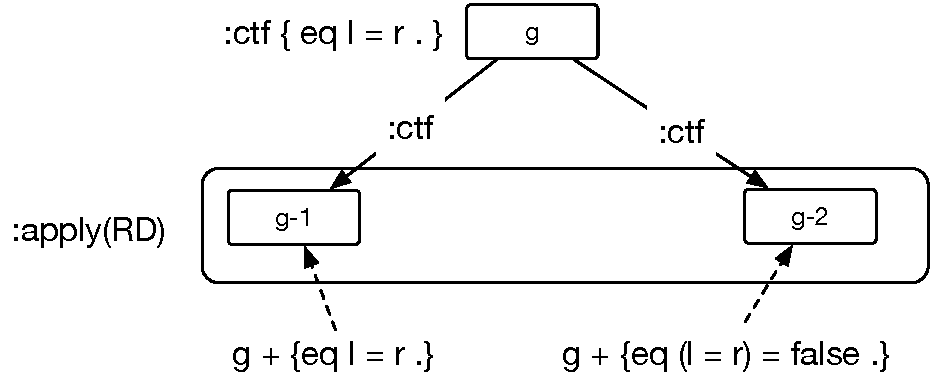
\includegraphics[scale=0.6]{ctf.pdf}
  \caption{:ctf の動作}
  \label{fig:ctf}
\end{figure}
\paragraph{図\ref{fig:ctf} の説明}
 ゴール g が現在のターゲットゴールとする.この状態で
  \begin{simplev}
    :ctf {eq l = r . }
  \end{simplev}
  とすると,ゴール g に \texttt{eq l = r .} を仮定として追加した g-1 (true の場合)と,
  \texttt{eq (l = r) = false .} を追加した g-2 (false の場合)を作成し,
  ゴール g の子ゴールとする.
  その後,g-1 と g-2 のそれぞれに対して戦略 RD を適用する.

\subsection{:csp コマンド}\label{sec:csp}
\texttt{:ctf} コマンドは複数の等式または遷移規則を指定し,
各々が成立するとした小ゴールを作成する.
その後,各小ゴールに対して暗黙的に戦略 RD (\ref{sec:RD}) を適用する.

\begin{itemize}
\item 構文
  \begin{vvtm}
    \begin{simplev}
      ケース指定分割 ::= :csp "{" { <Equation> . | <Transition> .}+ "}"
    \end{simplev}
  \end{vvtm}
\end{itemize}

\begin{figure}[hbt]
  \centering
  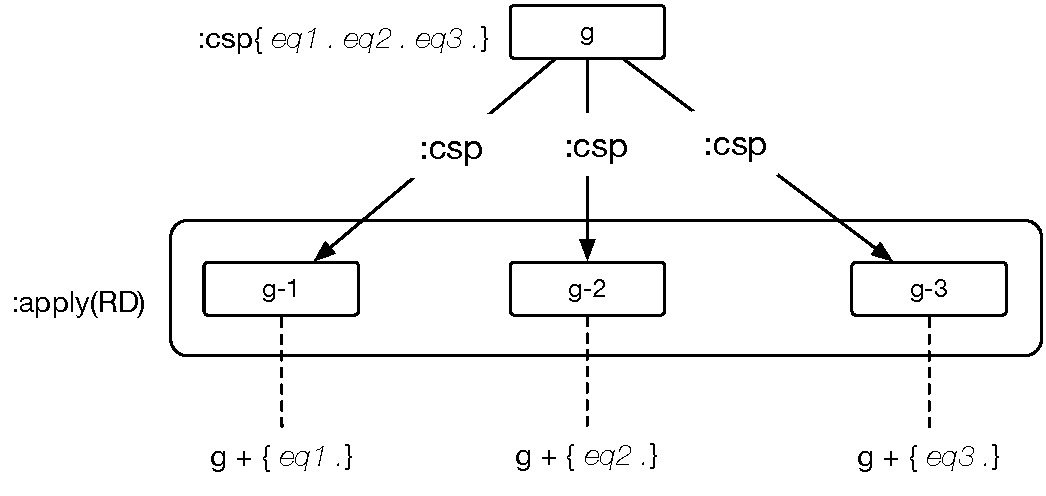
\includegraphics[scale=0.6]{csp.pdf}
  \caption{:csp の動作}
  \label{fig:csp}
\end{figure}

\paragraph{図~\ref{fig:csp}の説明}
ターゲットゴールが g だとする.”:csp { \textit{eq1} . \textit{eq2} . \textit{eq3} . }” のようにして
3つの等式 eq1, eq2, および eq3 を指定した場合,:csp は3個の小ゴール g-1, g-2, g-3 を生成し,
それぞれに対して一つづつ指定された等式を配分する.
その後これらの小ゴールに対して暗黙的に戦略 RD を適用する.

\subsection{:show コマンド}
証明の進行状況などを確認するために有用と思われる情報をみるため,
既存の show コマンドと類似の機能を提供する \texttt{:show} コマンドを提供する.

\subsubsection{ゴール内容の表示 -- :show goal}
\begin{itemize}
\item ゴールの内容を表示する.
\item 構文
  \begin{vvtm}
    \begin{simplev}
    ゴールの表示 ::= :show goal [ <GoalName> ]
  \end{simplev}
\end{vvtm}
\item \verb|<GoalName>| で指定したゴールを表示する.
\item \verb|<GoalName>| が省略された場合は,現在のターゲット・ゴールを表示する.
\end{itemize}

\subsubsection{未証明のゴールの表示 -- :show unproved}
\begin{itemize}
\item 現時点でまだ証明されていないゴールを表示する.
\item 未証明のゴールとは,現在の証明過程における証明木で,末端のノードうち
  まだ証明対象の文が discharge されていないゴールの事を言う.
\item 構文
  \begin{vvtm}
    \begin{simplev}
      未証明のゴール表示 ::= :show unproved
    \end{simplev}
  \end{vvtm}
\end{itemize}

\subsubsection{証明木の構造表示 -- :show/:describe  proof}

\paragraph{:show proof}
\begin{itemize}
\item 現時点における証明木の構造を図式的に表示する.
\item 構文
  \begin{vvtm}
    \begin{simplev}
   証明木の表示 ::= :show proof
    \end{simplev}
  \end{vvtm}
\item 証明木の表示にあったっては,以下の事が容易に判別出来るようにする.
  \begin{itemize}
  \item ゴールがどの戦略によって生成されたものであるか
  \item ターゲット・ゴールが何であるか
  \item ゴールは証明済みか否か
  \end{itemize}
\end{itemize}

\paragraph{:describe proof}
\begin{itemize}
\item \verb|show proof| と同様だが図式的な構造の表示では無く,証明の過程で
  使用された演繹に関する情報を提示するのが目的である.
\item 構文
  \begin{vvtm}
    \begin{simplev}
   証明過程の表示 ::= :describe proof
    \end{simplev}
  \end{vvtm}
\item 表示にあたっては,以下の情報を提示する.
  \begin{itemize}
  \item そのゴールを生成した戦略
  \item 証明すべき文
  \item 帰納法の対象とした変数
  \item SI あるいは TC 戦略を適用するにあたって導入された定数
  \item 戦略によって導入された公理
  \item ゴールが証明されているか否か
  \end{itemize}
\end{itemize}


%%%%%%%%%%%%%%%%%%%%%%%%%%%%%%%%%%%%%%%%%%%%%%%%%%%%%%%%%%%%%%%%%%%%%%%%%%%%%%%%%%%%
\chapter{例題}
\label{chap:prototype}

本章では~\ref{chap:new-commands}で説明した CITP for Cafe の基本的な機能を網羅した例題について,
その実行例と合わせて説明する.

\section{足し算の性質の帰納法による証明}
\label{sec:pnat}
ペアノ流の自然数の上で足し算を定義し,足し算の交換則と結合則が成り立つことを証明する.

\subsubsection{PNATの定義}
自然数のソートは \texttt{PNat} とし,下位ソートとして \texttt{PZero} (ゼロ)と
\texttt{PNzNat} (1以上の自然数)を定義する.足し算は \texttt{+},
\texttt{0} と \texttt{s} が構成子である.
\begin{vvtm}
\begin{simplev}
**
** Prove associativity and commutativity of addition
** using CITP for CafeOBJ
**

mod! PNAT {
  [ PZero PNzNat < PNat ]
  op 0 : -> PZero {ctor} .
  op s_ : PNat -> PNzNat {ctor} .
  op _+_ : PNat PNat -> PNat .
  eq 0 + N:PNat = N .
  eq s M:PNat + N:PNat = s(M + N) .
}
\end{simplev}
\end{vvtm}

\subsection{準備}

結合則の証明に必要な性質として次の性質がある.

\begin{verbatim}
       N:PNat + 0 = N:PNat  .
       M:PNat + s N:PNat = s(M:PNat + N:PNat) .
\end{verbatim}

そのため,まず最初に足し算\texttt{+}で,これらの性質を先に証明する.
CIT for Cafe で証明するため,最初に PNAT を文脈として設定してから
証明したいゴールを設定する.

\begin{vvtm}
\begin{simplev}
select PNAT .
:goal { eq [lemma-1]: M:PNat + 0 = M:PNat .
        eq [lemma-2]: M:PNat + s N:PNat = s(M:PNat + N:PNat). }
\end{simplev}
\end{vvtm}

上の \texttt{:goal} コマンドの実行結果は次のようになる.
\begin{vvtm}
  \begin{simplev}
:goal { ** root -----------------------------------------
  -- context module: PNAT
  -- axioms to be proved
    eq [lemma-1]: M:PNat + 0 = M .
    eq [lemma-2]: M:PNat + s N:PNat = s (M + N) .
}
** Initial goal (root) is generated. **
  \end{simplev}
\end{vvtm}
ゴール名が \texttt{root} であり,先に \texttt{:goal} コマンドで指定した文が
証明対象となっている事が示されている.

証明は変数 \texttt{M:PNat} の上の帰納法によって行う.そのため \texttt{:ind on} コマンドで
帰納法で使用する変数を宣言する.証明の過程で生成されるゴールを確認したいため
\texttt{:verbose} コマンドで \texttt{on} を指定する.
デフォルトでは \texttt{:verbose} の値は \texttt{off} である.
\begin{vvtm}
\begin{simplev}
:ind on (M:PNat)

**> We want to see every goal generated in proof process.
:verbose on 
\end{simplev}
\end{vvtm}
上を実行するとシステムは \texttt{M} の上で帰納法を用いた証明を実施する旨表示する.
\begin{vvtm}
  \begin{simplev}
    **> Induction will be conducted on M:PNat 
  \end{simplev}
\end{vvtm}


証明は戦略 \texttt{:auto} で行う.これは戦略 \texttt{(SI CA TC IP RD)} と等価である.

\begin{vvtm}
\begin{simplev}
:auto 
\end{simplev}
\end{vvtm}

以下順次,\texttt{:auto} コマンドの出力を示す.
\begin{vvtm}
  \begin{simplev}
[si]=> :goal{root}
** Generated 2 goals
[si]=>
:goal { ** 1 -----------------------------------------
  -- context module: PNAT
  -- induction variable
    M:PNat
  -- axioms to be proved
    eq [lemma-1]: 0 + 0 = 0 .
    eq [lemma-2]: 0 + s N:PNat = s (0 + N) .
}
[si]=>
:goal { ** 2 -----------------------------------------
  -- context module: PNAT
  -- induction variable
    M:PNat
  -- constant for induction
    op M#PNat : -> PNat { prec: 0 }
  -- introduced axioms
    eq [SI lemma-1]: M#PNat + 0 = M#PNat .
    eq [SI lemma-2]: M#PNat + s N:PNat = s (M#PNat + N) .
  -- axioms to be proved
    eq [lemma-1]: s M#PNat + 0 = s M#PNat .
    eq [lemma-2]: s M#PNat + s N:PNat = s (s M#PNat + N) .
}
\end{simplev}
\end{vvtm}
まず最初に戦略 \texttt{si} が適用され,2つのゴールが生成されている.
ゴール 1 は帰納法のベースケースであり,もとの証明対象の文にあった
帰納法の変数 M を構成子 0 とした文が証明対象となる.

ゴール 2 はステップケースである.帰納法の仮定として,``ある自然数 N で
成り立つとしたとき'' に相当する文が導入されている.ある自然数 N に相当する
項のために定数 \verb|M#PNat| が使われている.この定数を定義するために
導入されたオペレータ宣言についてもゴールの表示で示されている.

証明対象とする文は,上で述べた仮定が成り立つとした時に示すべき文である.
そのため構成子 \texttt{s} により \verb|M#PNat| が展開されている.

戦略 si を適用したあと,システムは ca を自動的に適用する.
ca はまず最初にゴール1に対して適用される.
複数の証明対象がゴールに含まれているため,
それぞれを別々の子ゴールに分配し,それぞれでケース分けが
可能かどうかを調べる.
この場合ケースわけは実行されなかった(ケースわけの対象とする
公理は宣言されていない).

ca はケースわけ分析が終了した後に,暗黙的に文の充足性(ST)と
矛盾の有無(CT)を調べるが,その結果一つの文が充足されており
その旨出力する.具体的な出力は次のようになる.

\begin{vvtm}
\begin{simplev}
[ca]=> :goal{1}
[ca] discharged: eq [lemma-1]: 0 = 0

** Generated 2 goals
[ca]=>
:goal { ** 1-1 -----------------------------------------
  -- context module: PNAT
  -- discharged axiom
    eq [ST lemma-1]: 0 = 0 .
  -- induction variable
    M:PNat
} << proved >>
[ca]=>
:goal { ** 1-2 -----------------------------------------
  -- context module: PNAT
  -- induction variable
    M:PNat
  -- axiom to be proved
    eq [lemma-2]: 0 + s N:PNat = s (0 + N) .
}
\end{simplev}
\end{vvtm}

ca はゴール 1 の処理を終了後,残っているゴール2を対象ととして処理を続ける.
その実行の様子は次のようになる.
ここでも複数の証明対象を別々の小ゴールに分割してから,
それぞれでケース分け処理を実施する.
やはりケースわけは無く,処理の終わりで実施する ST + CT で,
ゴール 2-1 が discharge されている.

\begin{vvtm}
\begin{simplev}
[ca]=> :goal{2}
[ca] discharged: eq [lemma-1]: (s M#PNat) = (s M#PNat)
** Generated 2 goals
[ca]=>
:goal { ** 2-1 -----------------------------------------
  -- context module: PNAT
  -- discharged axiom
    eq [ST lemma-1]: s M#PNat = s M#PNat .
  -- induction variable
    M:PNat
  -- constant for induction
    op M#PNat : -> PNat { prec: 0 }
  -- introduced axioms
    eq [SI lemma-1]: M#PNat + 0 = M#PNat .
    eq [SI lemma-2]: M#PNat + s N:PNat = s (M#PNat + N) .
} << proved >>
[ca]=>
:goal { ** 2-2 -----------------------------------------
  -- context module: PNAT
  -- induction variable
    M:PNat
  -- constant for induction
    op M#PNat : -> PNat { prec: 0 }
  -- introduced axioms
    eq [SI lemma-1]: M#PNat + 0 = M#PNat .
    eq [SI lemma-2]: M#PNat + s N:PNat = s (M#PNat + N) .
  -- axiom to be proved
    eq [lemma-2]: s M#PNat + s N:PNat = s (s M#PNat + N) .
}
\end{simplev}
\end{vvtm}

この時点で残っているゴールは 1-2 と 2-2 である.
未だ適用されていない戦略 (TC IP RD) がこの順にこれらに対して
適用されていく.

TCは証明対象の文に含まれる変数を全て定数に置き換え,
その後結果となった文の充足性(ST)と矛盾の有無(CT)を調べる.
下の実行例ではまず残ったゴール1-2に対してこれが実施され,
文が充足されていることが確認できている.

\begin{vvtm}
\begin{simplev}
[tc]=> :goal{1-2}
[rd] discharged: 
  eq [TC lemma-2]: s N@PNat = s N@PNat
[tc] discharged the goal "1-2-1"
** Generated 1 goal
[tc]=>
:goal { ** 1-2-1 -----------------------------------------
  -- context module: PNAT
  -- discharged axiom
    eq [RD TC lemma-2]: s N@PNat = s N@PNat .
  -- induction variable
    M:PNat
  -- introduced constant
    op N@PNat : -> PNat { prec: 0 }
} << proved >>
\end{simplev}
\end{vvtm}

tc は続いてゴール2-2をターゲットとして実行するが,
同様に変数を定数に置き換えた結果の証明対象の文が
充足されるか,またゴール内の矛盾の有無を調べ,
ここでも文が充足されることが確認できている.

この時点で,ほかに証明対象とすべきゴールが存在しないため,
残りの戦略 (IP RD) は適用されない.
システムは全てのゴールが discharge され,
当初の証明対象が証明できたことを印字して,
:auto コマンドの処理を終了する.
実行の様子は次の通りである.

\begin{vvtm}
\begin{simplev}
[tc]=> :goal{2-2}
[rd] discharged: 
  eq [TC lemma-2]: s (s (M#PNat + N@PNat))
      = s (s (M#PNat + N@PNat))
[tc] discharged the goal "2-2-1"
** Generated 1 goal
[tc]=>
:goal { ** 2-2-1 -----------------------------------------
  -- context module: PNAT
  -- discharged axiom
    eq [RD TC lemma-2]: s (s (M#PNat + N@PNat))
        = s (s (M#PNat + N@PNat)) .
  -- induction variable
    M:PNat
  -- introduced constant
    op N@PNat : -> PNat { prec: 0 }
  -- constant for induction
    op M#PNat : -> PNat { prec: 0 }
  -- introduced axioms
    eq [SI lemma-1]: M#PNat + 0 = M#PNat .
    eq [SI lemma-2]: M#PNat + s N:PNat = s (M#PNat + N) .
} << proved >>
** All goals are successfully discharged.

  \end{simplev}
\end{vvtm}

以上の証明において,戦略が適用されどのようにゴールが生成されたかは,
\verb|show proof| コマンドによってみることが出来る.
下に実行例を示す.

\begin{vvtm}
  \begin{simplev}
PNAT> show proof
                    root*                     
          /                       \            
       [si] 1*                 [si] 2*        
    /           \           /           \      
[ca] 1-1*   [ca] 1-2*   [ca] 2-1*   [ca] 2-2* 
                |                       |      
           [tc] 1-2-1*             [tc] 2-2-1*

  \end{simplev}
\end{vvtm}

\subsection{交換則と結合則の証明}
引き続いて,足し算 \texttt{+} の交換則と結合則を証明する.
これら証明には先に証明した lemma-1 と lemma-2 が必要である.
そのためこれらを公理として導入した新たなモジュール PNAT-L を宣言する.

\begin{vvtm}
  \begin{simplev}
mod! PNAT-L {
  inc(PNAT)
  eq [lemma-1]: N:PNat + 0 = N .
  eq [lemma-2]: M:PNat + s N:PNat = s(M + N). 
}
  \end{simplev}
\end{vvtm}

\subsubsection{交換則の証明}

まず最初に交換則を証明する.PNAT-L を文脈として設定し,
ゴールを宣言する.
\begin{vvtm}
  \begin{simplev}
open PNAT-L .
:goal { eq M:PNat + N:PNat = N:PNat + M:PNat . }
  \end{simplev}
\end{vvtm}
今度は文脈の設定に select ではなく,open を用いた.
実行結果は次のようになる.
\begin{vvtm}
  \begin{simplev}
-- opening module PNAT-L.. done.

:goal { ** root -----------------------------------------
  -- context module: %
  -- axiom to be proved
    eq M:PNat + N:PNat = N + M .
}
** Initial goal (root) is generated. **
  \end{simplev}
\end{vvtm}

証明は帰納法を用いるため,帰納法で使用する変数を指定する.
\begin{vvtm}
  \begin{simplev}
%PNAT-L> :ind on (M:PNat)
**> Induction will be conducted on M:PNat 
  \end{simplev}
\end{vvtm}

戦略として今回は :auto ではなく,陽に戦略を指定し :apply コマンドによって証明を試みる.
まず最初に SI コマンドによって帰納法のベースケースとステップケースに相当するゴールを
作成する.

\begin{vvtm}
  \begin{simplev}
%PNAT-L> :apply (SI)

[si]=> :goal{root}
** Generated 2 goals
[si]=>
:goal { ** 1 -----------------------------------------
  -- context module: %
  -- induction variable
    M:PNat
  -- axiom to be proved
    eq 0 + N:PNat = N + 0 .
}
[si]=>
:goal { ** 2 -----------------------------------------
  -- context module: %
  -- induction variable
    M:PNat
  -- constant for induction
    op M#PNat : -> PNat { prec: 0 }
  -- introduced axiom
    eq [SI]: M#PNat + N:PNat = N + M#PNat .
  -- axiom to be proved
    eq s M#PNat + N:PNat = N + s M#PNat .
}
>> Next target goal is "1".
>> Remaining 2 goals.
  \end{simplev}
\end{vvtm}

上のように2つのゴールが生成された.
現在の証明木は次のようになっている.
\begin{vvtm}
  \begin{simplev}
%PNAT-L> show proof
     root      
   /        \   
>[si] 1  [si] 2
  \end{simplev}
\end{vvtm}

デフォルトで次の戦略の適用対象となるゴールには,証明木のノードに
\verb|>| と表示してそれと分かるようになっている.
次に適用する戦略として TC を選択した例を下に示す.

\begin{vvtm}
  \begin{simplev}
%PNAT-L> :apply (tc)
[tc]=> :goal{1}
[rd] discharged: 
  eq [TC]: N@PNat = N@PNat
[tc] discharged the goal "1-1"
** Generated 1 goal
[tc]=>
:goal { ** 1-1 -----------------------------------------
  -- context module: %
  -- discharged axiom
    eq [RD TC]: N@PNat = N@PNat .
  -- induction variable
    M:PNat
  -- introduced constant
    op N@PNat : -> PNat { prec: 0 }
} << proved >>
>> Next target goal is "2".
>> Remaining 1 goal.

%PNAT-L> sh proof
       root       
    /         \    
 [si] 1*   >[si] 2
    |              
[tc] 1-1*        
  \end{simplev}
\end{vvtm}
dischage する事が出来た.証明木のノードに \verb|*| が付加されているのは
それが discharge されている事を示したものである.

残りのゴール 2 に対しても TC で証明を試みる.結果は次のようになる.
\begin{vvtm}
  \begin{simplev}
%PNAT-L> :apply (TC)
[tc]=> :goal{2}
[rd] discharged: 
  eq [TC]: s (N@PNat + M#PNat) = s (N@PNat + M#PNat)
[tc] discharged the goal "2-1"
** Generated 1 goal
[tc]=>
:goal { ** 2-1 -----------------------------------------
  -- context module: %
  -- discharged axiom
    eq [RD TC]: s (N@PNat + M#PNat) = s (N@PNat + M#PNat) .
  -- induction variable
    M:PNat
  -- introduced constant
    op N@PNat : -> PNat { prec: 0 }
  -- constant for induction
    op M#PNat : -> PNat { prec: 0 }
  -- introduced axiom
    eq [SI]: M#PNat + N:PNat = N + M#PNat .
} << proved >>
** All goals are successfully discharged.
  \end{simplev}
\end{vvtm}
これで,交換則の証明が完了した.

SI と TC は \verb|:apply (SI TC)| のようにして続けて自動で適用するようにできる.
この場合は,上の実施例のように TC を2度指定する必要はなくなる.
下の例ではシステムの印字を抑制するため \verb|:verbose off| としている.
\begin{vvtm}
  \begin{simplev}
%PNAT-L> :verbose off

%PNAT-L> :apply (SI TC)
[si]=> :goal{root}
** Generated 2 goals
[tc]=> :goal{1}
[rd] discharged: 
  eq [TC]: N@PNat = N@PNat
[tc] discharged the goal "1-1"
** Generated 1 goal
[tc]=> :goal{2}
[rd] discharged: 
  eq [TC]: s (N@PNat + M#PNat) = s (N@PNat + M#PNat)
[tc] discharged the goal "2-1"
** Generated 1 goal
** All goals are successfully discharged.
  \end{simplev}
\end{vvtm}

\subsubsection{結合則の証明}
これまでと同じく,結合則も帰納法を用いて証明する.
特に新たに説明が必要なものは使われていないため,
\verb|:verbose off| として :auto で実行した例を下に示す.
\begin{vvtm}
  \begin{simplev}
%PNAT-L> :goal {eq (M:PNat + N:PNat) + P:PNat  = N:PNat + (M:PNat + P:PNat) . }
:goal { ** root -----------------------------------------
  -- context module: %
  -- axiom to be proved
    eq (M:PNat + N:PNat) + P:PNat = N + (M + P) .
}
** Initial goal (root) is generated. **
%PNAT-L> :ind on (M:PNat)
**> Induction will be conducted on M:PNat 
%PNAT-L> :auto
[si]=> :goal{root}
** Generated 2 goals
[cs]=> :goal{1}
[cs]=> :goal{2}
[tc]=> :goal{1}
[rd] discharged: 
  eq [TC]: N@PNat + P@PNat = N@PNat + P@PNat
[tc] discharged the goal "1-1"
** Generated 1 goal
[tc]=> :goal{2}
[rd] discharged: 
  eq [TC]: s (N@PNat + (M#PNat + P@PNat))
      = s (N@PNat + (M#PNat + P@PNat))
[tc] discharged the goal "2-1"
** Generated 1 goal
** All goals are successfully discharged.
%PNAT-L> show proof
       root*        
    /          \     
 [si] 1*    [si] 2* 
    |          |     
[tc] 1-1*  [tc] 2-1*
  \end{simplev}
\end{vvtm}

\section{場合分けによる証明}
先の証明の例は場合分けが必要となるものではなかった.
ここでは戦略 CA を用いた場合分けによる証明を示す.

\subsection{モジュール FG-FUN と証明対象}

下にモジュール FG-FUN の定義を示す.
この例題は Maude の CITP システムの例題を CafeOBJ 用に書きなおしたものである.

\begin{vvtm}
  \begin{simplev}
mod! FG-FUN {
  pr(NAT)
  op F : Nat -> Nat 
  op G : Nat -> Nat
  ceq[CA-1]: F(X:Nat) = 5 if X <= 7 .
  ceq[CA-2]: F(X:Nat) = 1 if 8 <= X .
  ceq[CA-3]: G(Y:Nat) = 2 if Y <= 4 .
  ceq[CA-4]: G(Y:Nat) = 7 if 5 <= Y .
}
  \end{simplev}
\end{vvtm}

特に意味のないモジュール定義である.
4つの条件付き等式が宣言されているが,それらは \texttt{CA} で始まる
ラベルを持っている.これはシステムに対して,これらの等式は
場合分けのケースを網羅したものであり,これを用いて場合分けをするように
指示するものである.

証明対象とする文は次の通りである.
\begin{vvtm}
  \begin{simplev}
9 <= G(F(X:Nat)) + G(X:Nat) = true
  \end{simplev}
\end{vvtm}
いかなる時もこれが成立することを示すのが目標である.
上の証明対象文に含まれている $F(X:Nat)$ と $G(X:Nat)$について, 
それぞれが公理で宣言された 2 つのケースを持つため,
可能なケースの組み合わせは表~\ref{tab:cases}のようになるはずである.
\begin{table}
\label{tab:cases}
\caption{可能な場合分けの組み合わせ}
\begin{center}
\begin{tabular}[htb]{|c|c|c|}\hline
&$F(X:Nat)$ & $G(X:Nat)$ \\\hline
(1)&$X \le 7$ & $X \le 4$ \\
(2)&$X \le 7$ & $5 \le X$ \\
(3)&$8 \le X$ & $X \le 4$ \\
(4)&$8 \le X$ & $5 \le X$ \\\hline 
\end{tabular}
\end{center}
\end{table}

これらの組み合わせのうち,(3) のケースは
X が 8 以上かつ 4 以下という条件のためあり得ない.
従ってシステムはこの組み合わせについてはこれを検知し,
当該の条件を含むゴールを discharge できなければならない.

\subsection{CITP for Cafe による証明}

先に示したモジュール FG-FUN を文脈として証明を実施した例を以下に示す.
個々の戦略の適用で作成されたゴールを見たいため,\verb|:verbose on| として実施した.

\begin{vvtm}
  \begin{simplev}
FG-FUN> :goal { eq 9 <= G(F(X:Nat)) + G(X:Nat) = true . }

:goal { ** root -----------------------------------------
  -- context module: FG-FUN
  -- axiom to be proved
    eq 9 <= (G(F(X:Nat)) + G(X)) = true .
}
** Initial goal (root) is generated. **
  \end{simplev}
\end{vvtm}

上記のゴールに対して場合分けによる証明を行う.
使用する戦略は (CA TC RD) である.
以下システムの出力を幾つかに分割し,必要な説明を間に付加する形で示す.

\begin{vvtm}
  \begin{simplev}
FG-FUN> :apply (TC CA RD)

[tc]=> :goal{root}
** Generated 1 goal
[tc]=>
:goal { ** 1 -----------------------------------------
  -- context module: FG-FUN
  -- introduced constant
    op X@Nat : -> Nat { prec: 0 }
  -- axiom to be proved
    eq [TC]: 9 <= (G(F(X@Nat)) + G(X@Nat))
        = true .
}
\end{simplev}
\end{vvtm}
最初にゴール root に TC が適用され,証明対象とする文
\begin{verbatim}
    eq 9 <= (G(F(X:Nat)) + G(X)) = true .
\end{verbatim}
の \texttt{X} を \verb|X@Nat| に置き換えた文とした新たなゴール 1 を生成している.

次にこのゴール1に対して戦略 CA が適用され,先に見た4つのケース毎に
ゴールが生成されている.
CAはケースを新たな公理として導入後,それらの間に矛盾が無いかどうかを
チェックする.現在は暗黙的戦略 LE のみが実装されているが,
これによってゴール1-3が discharge されている.

\begin{vvtm}
\begin{simplev}
[ca]=> :goal{1}
[le] discharged the goal "1-3"
** Generated 4 goals
\end{simplev}
\end{vvtm}

以下ではシステムが生成した個々のゴールの内容をみる.

\begin{vvtm}
\begin{simplev}
[ca]=>
:goal { ** 1-1 -----------------------------------------
  -- context module: FG-FUN
  -- introduced constant
    op X@Nat : -> Nat { prec: 0 }
  -- introduced axioms
    eq [CA]: 5 <= X@Nat = true .
    eq [CA]: X@Nat <= 7 = true .
  -- axiom to be proved
    eq [TC]: 9 <= (G(F(X@Nat)) + G(X@Nat))
        = true .
}
\end{simplev}
\end{vvtm}
ゴール1-1は先の表~\ref{tab:cases}に示した(2)のケースに対応する.
文脈モジュール FG-FUN で宣言されていた公理
\begin{verbatim}
  ceq[CA-1]: F(X:Nat) = 5 if X <= 7 .
  ceq[CA-2]: F(X:Nat) = 1 if 8 <= X .
  ceq[CA-3]: G(Y:Nat) = 2 if Y <= 4 .
  ceq[CA-4]: G(Y:Nat) = 7 if 5 <= Y .
\end{verbatim}
のうち,CA-1 とCA-4 からこれらのケースが得られている.

\begin{vvtm}
\begin{simplev}
[ca]=>
:goal { ** 1-2 -----------------------------------------
  -- context module: FG-FUN
  -- introduced constant
    op X@Nat : -> Nat { prec: 0 }
  -- introduced axioms
    eq [CA]: 5 <= X@Nat = true .
    eq [CA]: 8 <= X@Nat = true .
  -- axiom to be proved
    eq [TC]: 9 <= (G(F(X@Nat)) + G(X@Nat))
        = true .
}
\end{simplev}
\end{vvtm}
ゴール 1-2 は表~\ref{tab:cases}のケース(4)に対応している.

\begin{vvtm}
\begin{simplev}
[ca]=>
:goal { ** 1-3 -----------------------------------------
  -- context module: FG-FUN
  -- discharged axiom
    eq [LE TC]: 9 <= (G(F(X@Nat)) + G(X@Nat))
        = true .
  -- introduced constant
    op X@Nat : -> Nat { prec: 0 }
  -- introduced axioms
    eq [CA]: X@Nat <= 4 = true .
    eq [CA]: 8 <= X@Nat = true .
} << proved >>
\end{simplev}
\end{vvtm}
ゴール1-3は表~\ref{tab:cases}のケース(3)に対応する.
先に述べたとおり,導入された公理は互いに矛盾するため,
システムはこのゴールを discharge している.
discharge された証明対象であった文は,
ゴールの表示上ラベル LE を追加した文として表示されている.

\begin{vvtm}
  \begin{simplev}
[ca]=>
:goal { ** 1-4 -----------------------------------------
  -- context module: FG-FUN
  -- introduced constant
    op X@Nat : -> Nat { prec: 0 }
  -- introduced axioms
    eq [CA]: X@Nat <= 4 = true .
    eq [CA]: X@Nat <= 7 = true .
  -- axiom to be proved
    eq [TC]: 9 <= (G(F(X@Nat)) + G(X@Nat))
        = true .
}
\end{simplev}
\end{vvtm}
CAが生成した最後にのゴール1-4は表~\ref{tab:cases}に示したケース
(1) に対応する.

以上のCAが生成した4つのゴールのうち,1個(1-3)は既に CA の
内部処理によって discharge されている.残りの3ゴールに対して
RD が適用される.RD が行うことは文の充足性検査と矛盾の検査であり,
暗黙的戦略 ST と CT を実施することと実質的に等価である.

\begin{vvtm}
\begin{simplev}
[rd]=> :goal{1-1}
[rd] discharged: 
  eq [TC]: 9 <= (G(F(X@Nat)) + G(X@Nat))
      = true
[rd] discharged goal "1-1".
[rd]=> :goal{1-2}
[rd] discharged: 
  eq [TC]: 9 <= (G(F(X@Nat)) + G(X@Nat))
      = true
[rd] discharged goal "1-2".
[rd]=> :goal{1-3}
[rd]=> :goal{1-4}
[rd] discharged: 
  eq [TC]: 9 <= (G(F(X@Nat)) + G(X@Nat))
      = true
[rd] discharged goal "1-4".
** All goals are successfully discharged.
  \end{simplev}
\end{vvtm}

上の実行例の通り,全てのゴールが満足されている.

以上の証明の結果に対応する証明木を表示すると次のようになる.
\begin{vvtm}
  \begin{simplev}
FG-FUN> show proof
                  root*                   
                    |                      
                 [tc] 1*                  
    /          |          |          \     
[ca] 1-1*  [ca] 1-2*  [ca] 1-3*  [ca] 1-4*
  \end{simplev}
\end{vvtm}
RD はゴールを生成しないため,証明木上で新たなノードは表示されていない.
結果を確認するため,ゴール1-1を表示してみると次のようになる.
\begin{vvtm}
  \begin{simplev}
FG-FUN> show goal 1-1
[ca]=>
:goal { ** 1-1 -----------------------------------------
  -- context module: FG-FUN
  -- discharged axiom
    eq [RD TC]: 9 <= (G(F(X@Nat)) + G(X@Nat))
        = true .
  -- introduced constant
    op X@Nat : -> Nat { prec: 0 }
  -- introduced axioms
    eq [CA]: 5 <= X@Nat = true .
    eq [CA]: X@Nat <= 7 = true .
} << proved >>
  \end{simplev}
\end{vvtm}
RD によって discharge された文は,ラベルに RD が追加されて表示される.
これによって,RD の適用による discharge であったことを知ることができる.

%%%%%%%%%%%%%%%%%%%%%%%%%%%%%%%%%%%%%%%%%%%%%%%%%%%%%%%%%%%%%%%%%%%%%%%%%%%%%%%%%%% 
\bibliographystyle{plain}
\bibliography{bib}
\end{document}
%%% Local Variables: 
%%% mode: latex
%%% TeX-master: t
%%% End: 
